\subsection{Evaluation}
We did not have the ability to do usability testing on medical personnel, if we had we would have done a combination of think out loud, and scenario testing, in order to determine if it would be useable, and fulfilling the requirements that we had set up.
Insted we did some small quantity tests our self.
This data can be used in a usability benchmark as the base line, if there are going to be futhere devoplement on it.

\subsubsection{Break Test}
We tested to see how much the record can handle before it breaks(See figure \ref{fig:BreakTest1}).
\begin{figure}[h]
	\begin{center}
	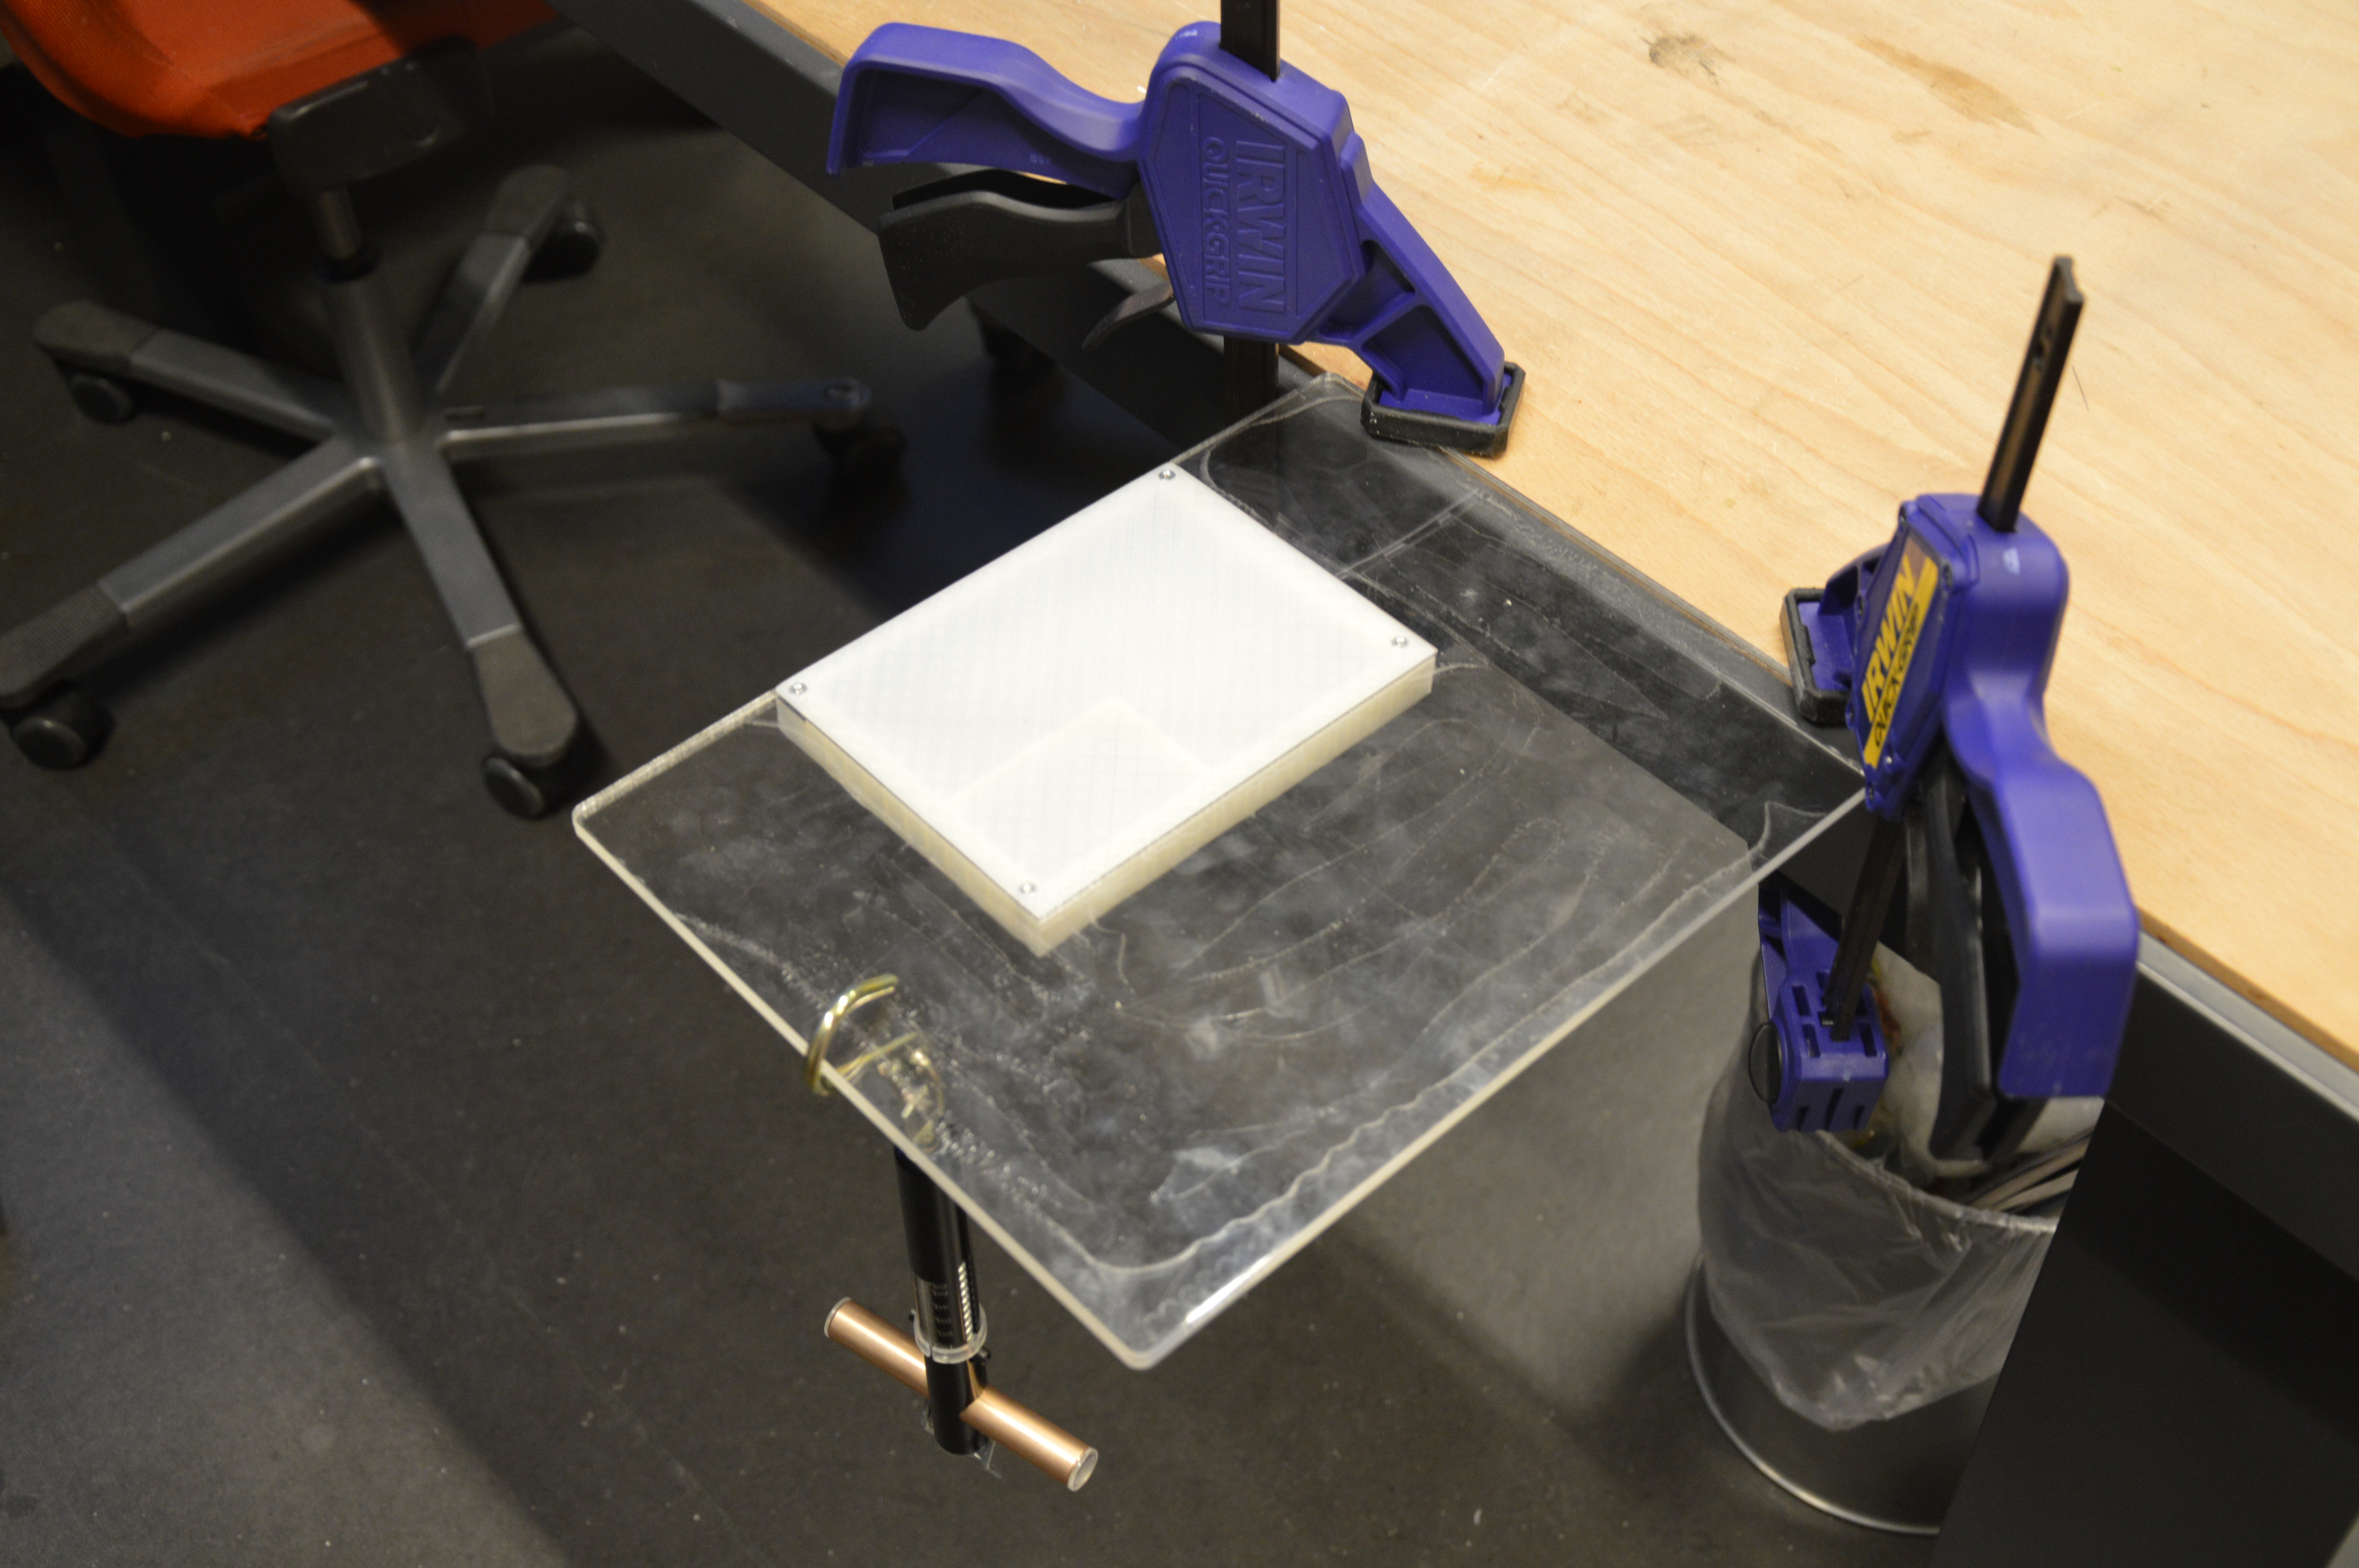
\includegraphics[scale=0.1]{images/DSC_0002.JPG}
	\caption{\small {\it {Test stepup}}} \label{fig:BreakTest1}
	\end{center}
\end{figure}
We did that by taking the weight in the workshop, that can measure kg. We put it on the far end of the acrylic, while the othere end was fastened to the table, and pushed down it measured that it can handle 7 kg of pressure before it breaks, one strange thing was that it did not break where we thought it would break, we sould have tougth that it would have broken in the sharp corner\cite{AcrylTension}, due to the tenssions that are build up there. We can see that it broke, further out from the center of the plate, as can be seen on figure\ref{fig:BreakTest2}.
\begin{figure}[h]
	\begin{center}
	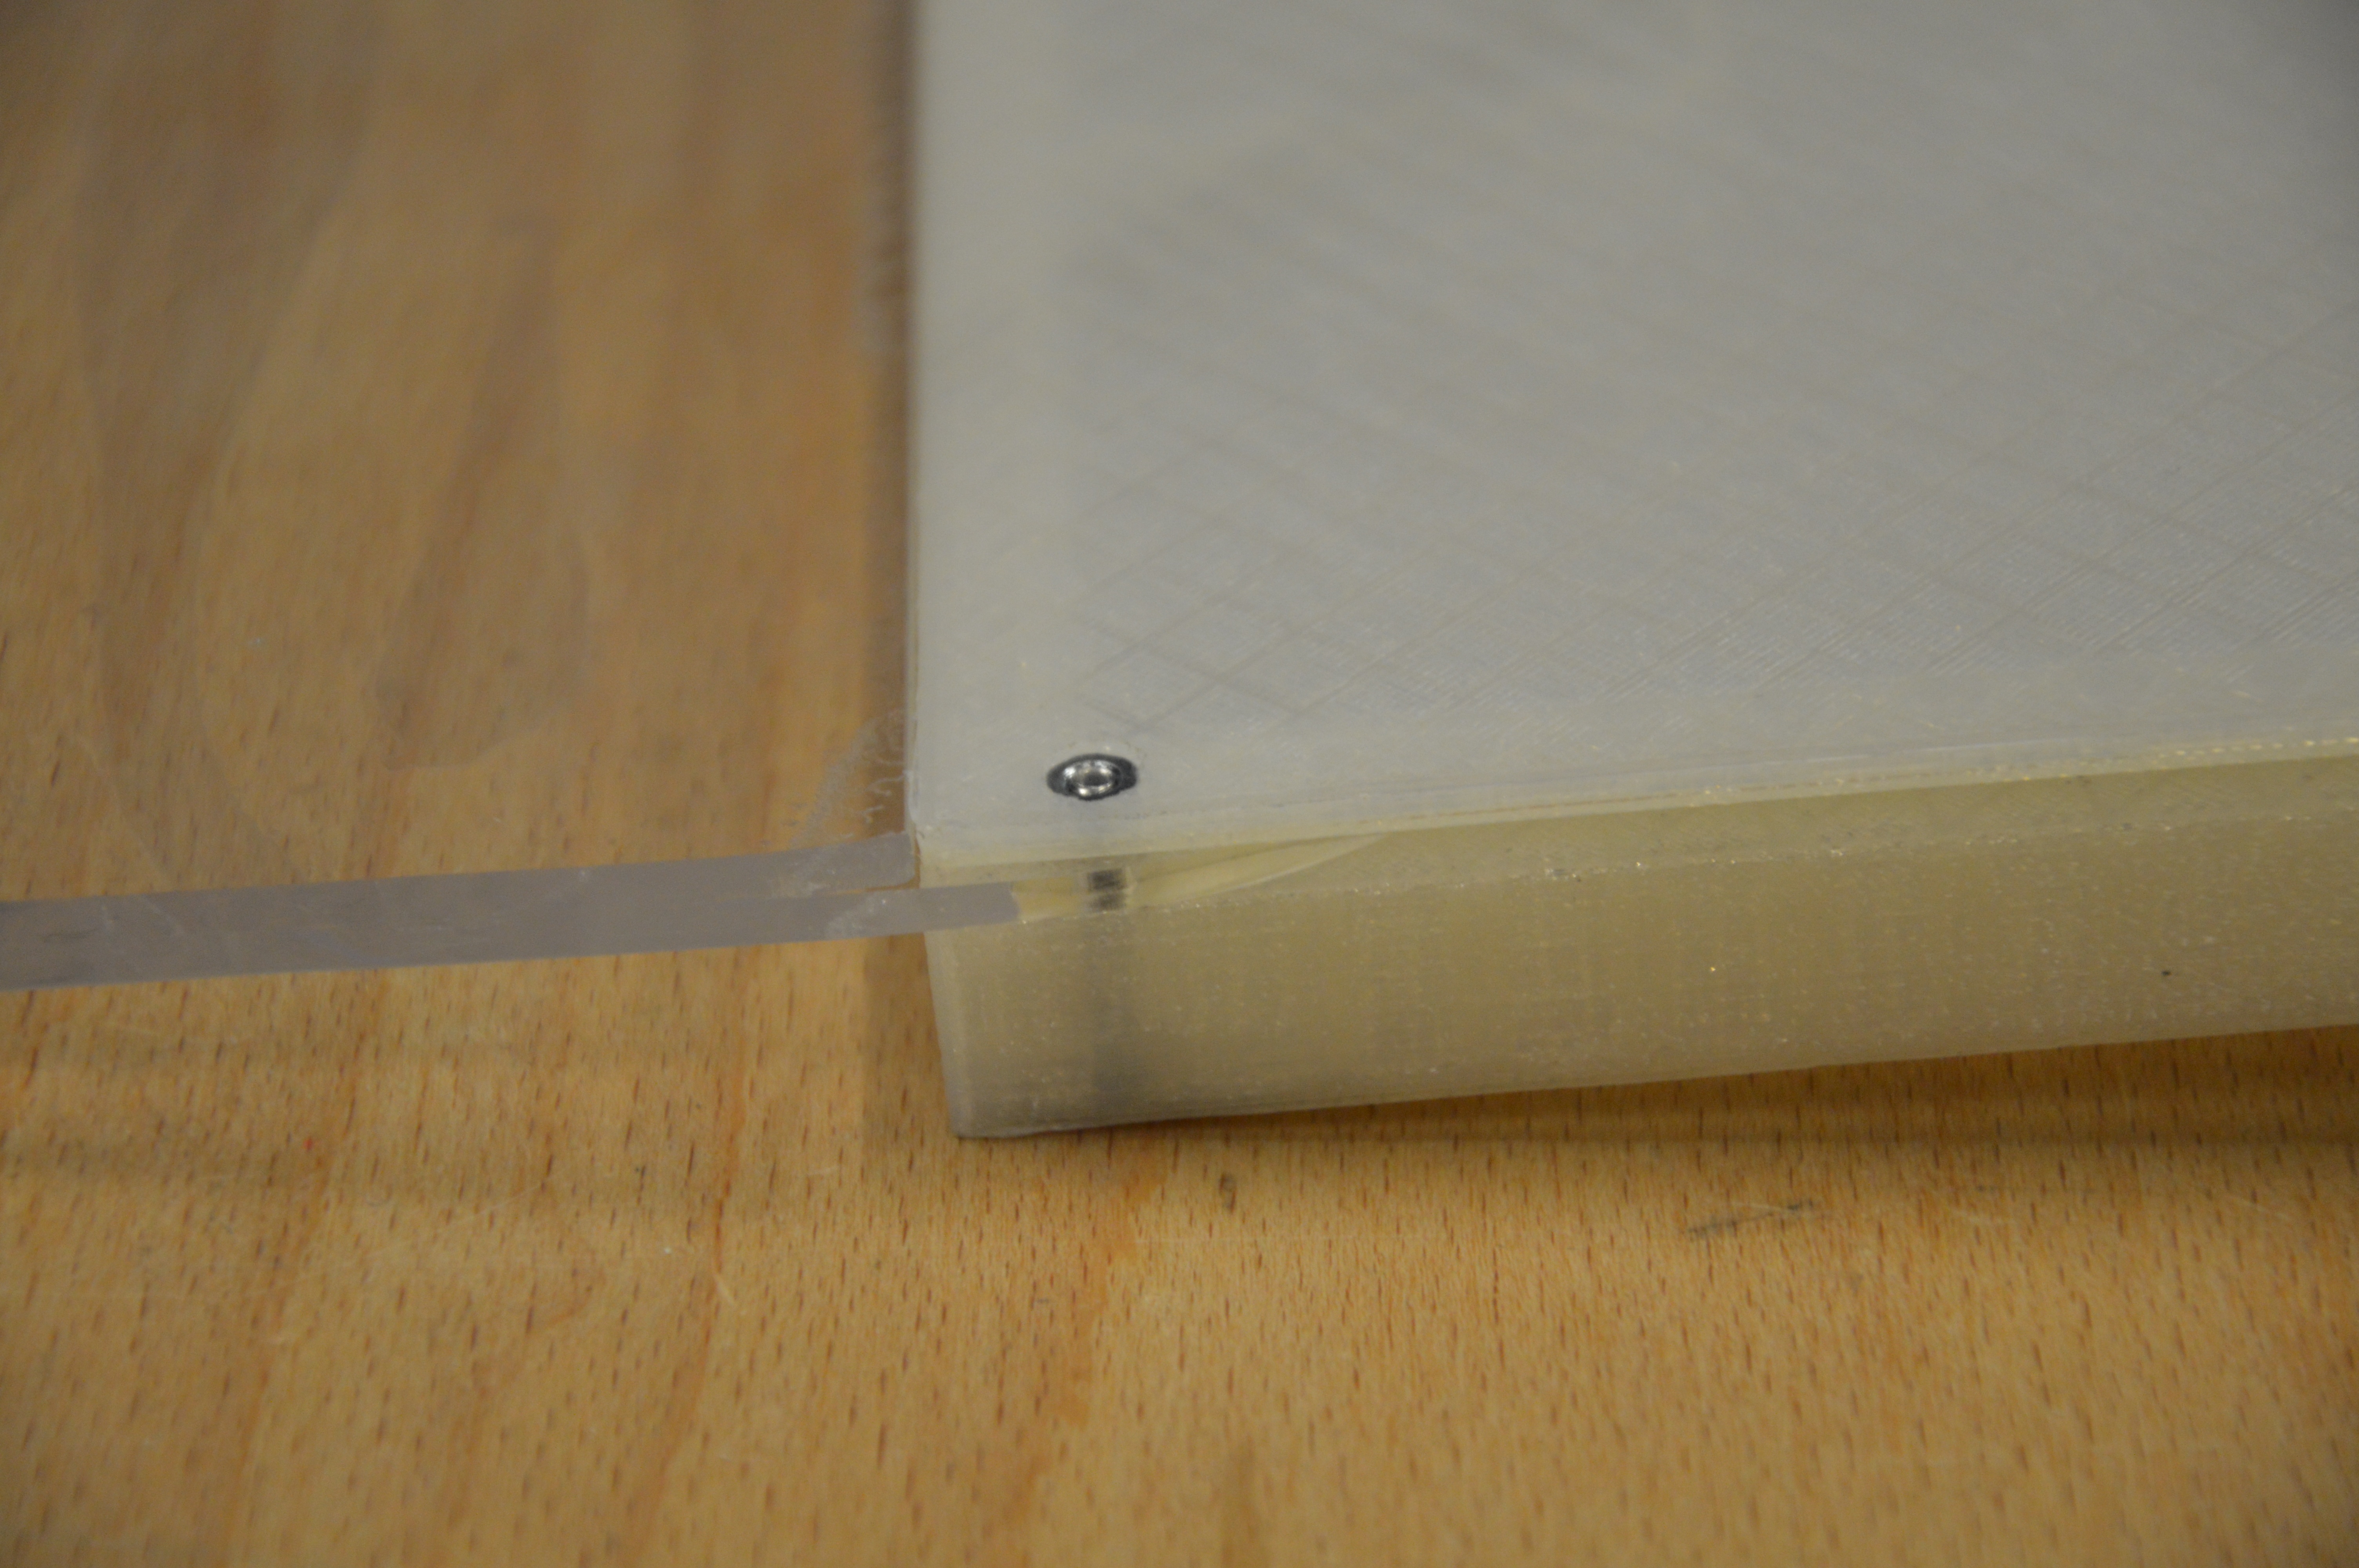
\includegraphics[scale=0.1]{images/DSC_0022.JPG}
	\caption{\small {\it {BreakTest}}} \label{fig:BreakTest2}
	\end{center}
\end{figure}
this might suggest that the box it self, is helping to give it strength, or that it just was weakest there, the glue might also have some thing to dio with it.
We can do this test over and over again, with different results, since we don't know what factor, that is in play.

newton stress meter test to record how the stresses are build up in the material, and how much.

\subsubsection{Drop Test}
We did testing on the last iteration of our design, where we drop at a distance of 1 meter 10 times to simulate the fall from a desk, after each time we locked for signs that it was about to crack or fracture.
After the 10'th drop we started to see cracks in the acrylic, the cracks appeared in the cutout section where there is a sharp corner, however this was only on the front acrylic plate, had we done the drop many more times we properly would have seen the same result in the back plate.
This is properly due to the laser cutting, and could be avoid by making a round cut rather that a sharp cut, or by drilling a hule to relieve tension there might have been build up, during the laser cutting.

We did not check the hardware during the drop test, after tests we checked the electronic and found that it hadn't suffered any damage.

For at better result to realy see what happend, we would have used a drop machine with a hign speed camara like the one that mensioned in article \cite{DropTest}, which is a machine that is buld for realistick drop test.
We could split it up, to see how many drops the box and plate can handle each.

\subsubsection{Power Test}
For the power test, we borrowed a discharger from Vaidas, where you can set the amount of amps it has to drain.
We calculated that all the devices would drain around 350 milliamps int total, if they run at maximum capacity, we found the information from the datasheets that are included for each device.
From the test where we put it on the discharger, we found out that it would run for 4 hours in the worst case, we later found out that if it is in idle mode, it can run for around 20 hours.

\subsubsection{Visual Test}
We tested if we were able to see the different LED colors, at a distance of 10 meter or more during the night and day, we made if shift between green, blue, red and yellow, throughout the test we had no problems seeing the led change, at distance over 20 meters, but for a better evaluation we would have like to have done a more technical approche like in artical \cite{LEDLIGHT}, where they used mathematical models in a simulation, in order to predict how the light was going to behave. That kind of data is easier to compair.

\subsubsection{Sound Test}
In order to see if we where able to find the record only by sound.
We set up some test senarios, 2 where it was out in the open, 2 where it was hidden under some object and 2 where it was inside an object. From the atarting point of the person in the test, there should be the same distance.
At each trail we did not find any major difference, whitch conclude that the speaker emitteda tone that was high enough to find it.
For better data to evaluate we could have messured the dB(disabel), to see how much it changed when put different places

\subsubsection{Price}
Since we had to keep it under 1000 kr pr device, we locked around on the internet, to finde the cheapest parts.
the price for the acrylic is taken from RIAS \cite{RIAS} where one 3mm thick $1 m^2$ acrylic is 532 kr.
\begin{itemize} \itemsep0em
	 \item WIFI: 191 kr \cite{Adafruit}
	 \item Arduino: 54 kr \cite{Sparkfun}
	 \item RFID: 112 kr \cite{Let-Eletronik}
	 \item Batterie: Courtesy of getvolt  \cite{Getvolt}
	 \item LED: 7 kr \cite{Adafruit}
	 \item Charger: Courtesy of getvolt \cite{Getvolt}
	 \item Stepup converter: Courtesy of getvolt  \cite{Getvolt}
	 \item Acryl: $(acrylic hight * acrylic width)*2 = 0,2 m^2 = 106.4 kr $ \cite{RIAS}
	 \item PLA: Weight times 0,33 
	 \item Total: 470,4 kr
\end{itemize}
If we had bought the stepup, charger and batteri we still would have been under the budgit limit.

\subsubsection{Conclusion}
The Data that we have from the evaluation, can be used as a to form for a simple benchmark for futhere evaluation.
So for futhere version the device should be able to handle more that 10 drops, be able to hold to more that 7 kg of force, the batterie life should be longere that 4-20 hours depending on it's use, the visability should still be no less that 10 meters, and the speaker should be loud enough, so it can be heard, even if it is hidden.
But one should propperly look away from the cost, since we have used sheap materials, compaiered to what is used i real medical devices, however on the othere side, it can be used, as a mark for how close othere iterations can come to the price.